%% ======================================================================
%% 07_build.tex -- 6. Build instructions
%% ======================================================================
\section{Build instructions}
\label{sec:build}

\paragraph{Tools}
\begin{itemize}
  \item hex keys and TETRIX wrenches;
  \item soldering iron, crimper for XT60 and Dupont connectors, multimeter, and DC clamp meter;
  \item FDM 3D printer (PLA, 0.2\,mm layer height, 30\% infill for the towers and linkages);
  \item a laptop with Arduino CLI (ESP32 core), PlatformIO, and LabVIEW 2019 with the myRIO Toolkit.
\end{itemize}

\paragraph{Safety}
Assemble and flash all boards with the LiPo batteries disconnected and propellers removed. Verify the spin direction of every motor without propellers before the first flight.

\begin{figure}[!htbp]
  \centering
  \begin{subfigure}[b]{0.24\textwidth}\centering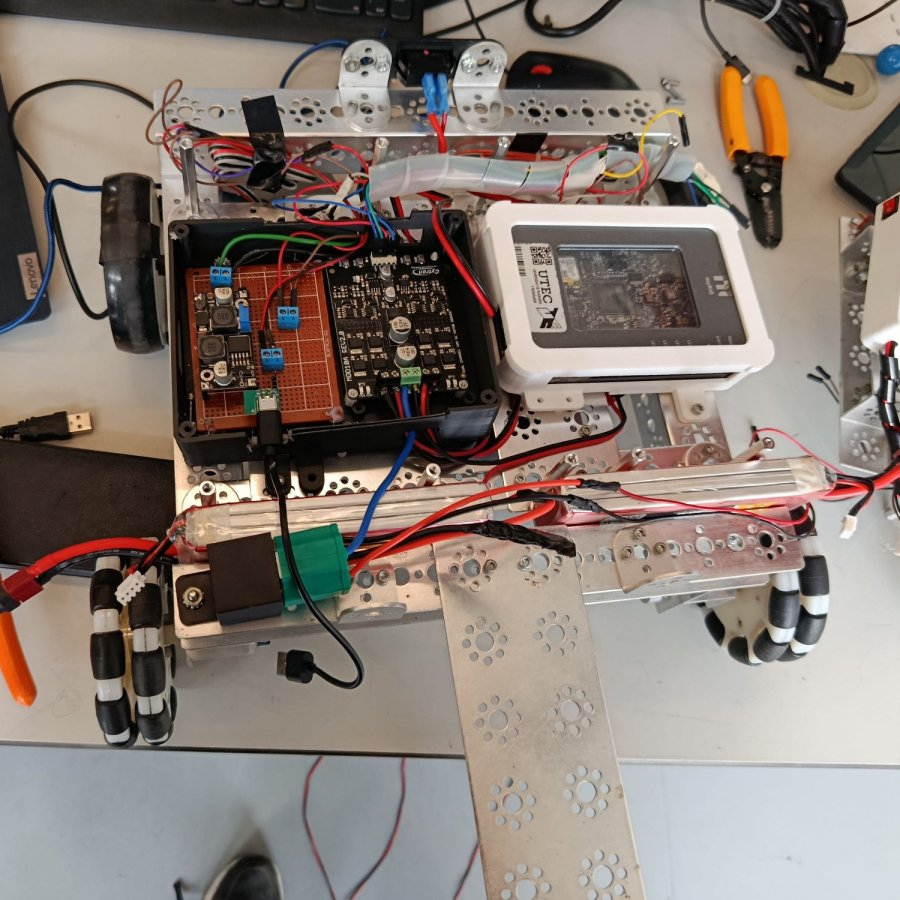
\includegraphics[width=\linewidth]{figures/paso1_base.jpg}\caption{Step 1: mobile base (myRIO, MDD10A, LiPo).}\end{subfigure}\hfill
  \begin{subfigure}[b]{0.24\textwidth}\centering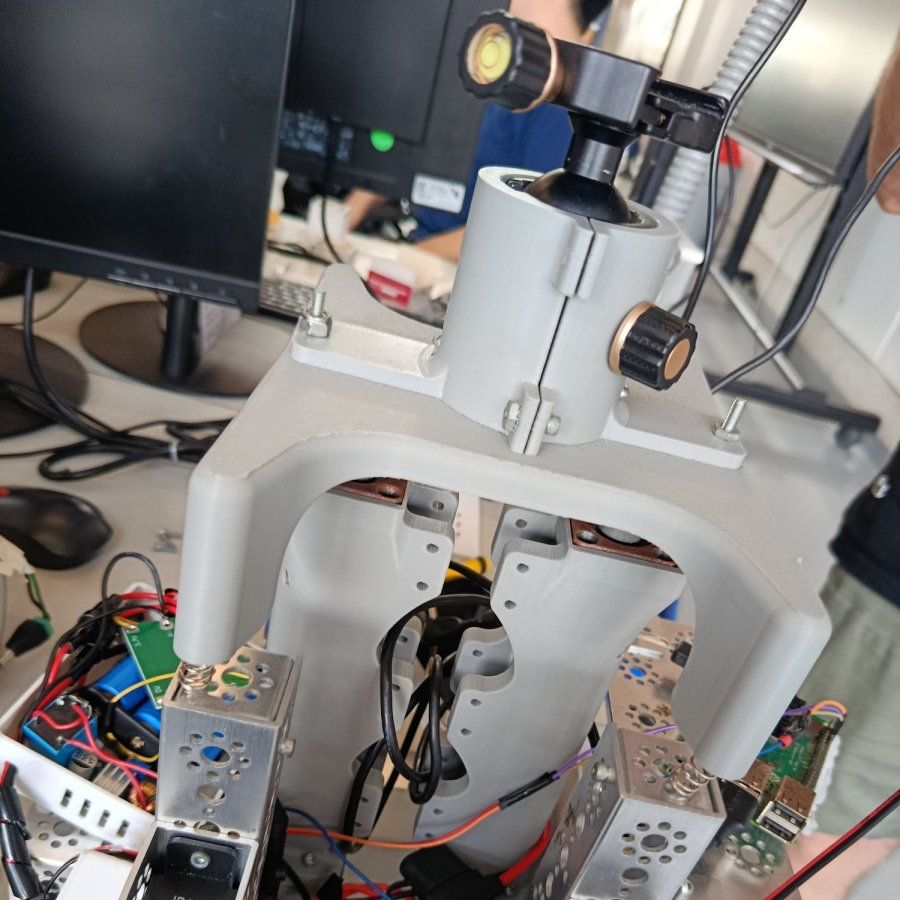
\includegraphics[width=\linewidth]{figures/paso2_mastil.jpg}\caption{Step 2: mast, guide, and spherical joint.}\end{subfigure}\hfill
  \begin{subfigure}[b]{0.24\textwidth}\centering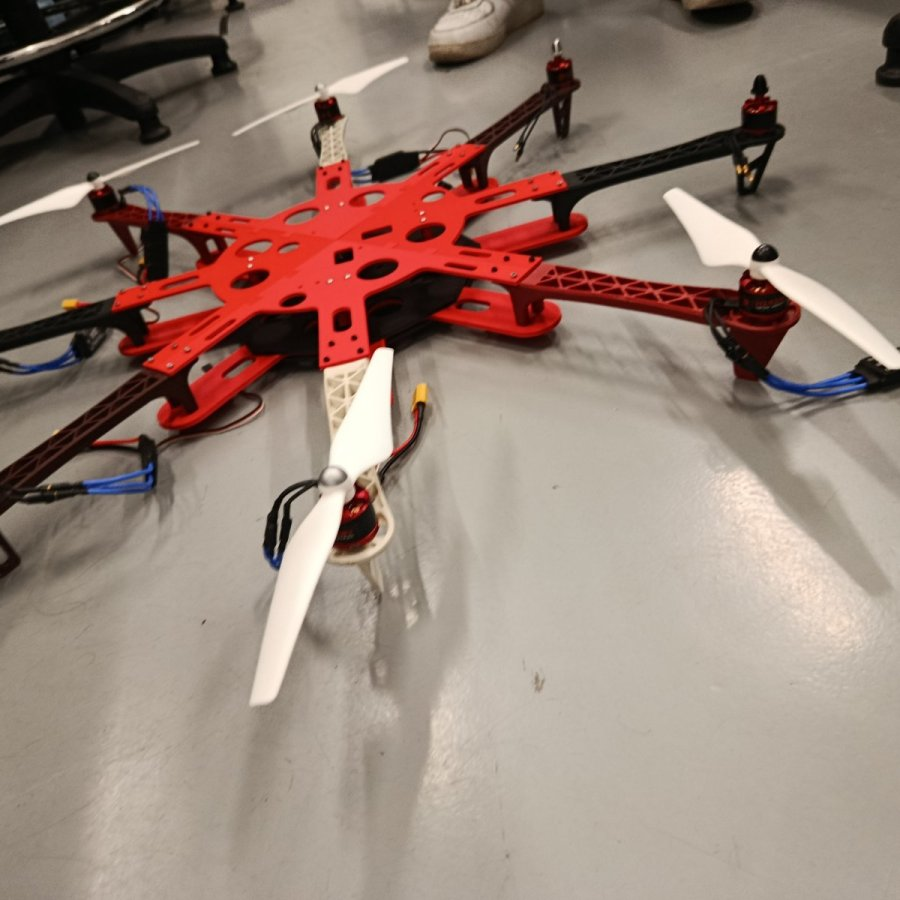
\includegraphics[width=\linewidth]{figures/paso3_marco.jpg}\caption{Step 3: eight-arm frame.}\end{subfigure}\hfill
  \begin{subfigure}[b]{0.24\textwidth}\centering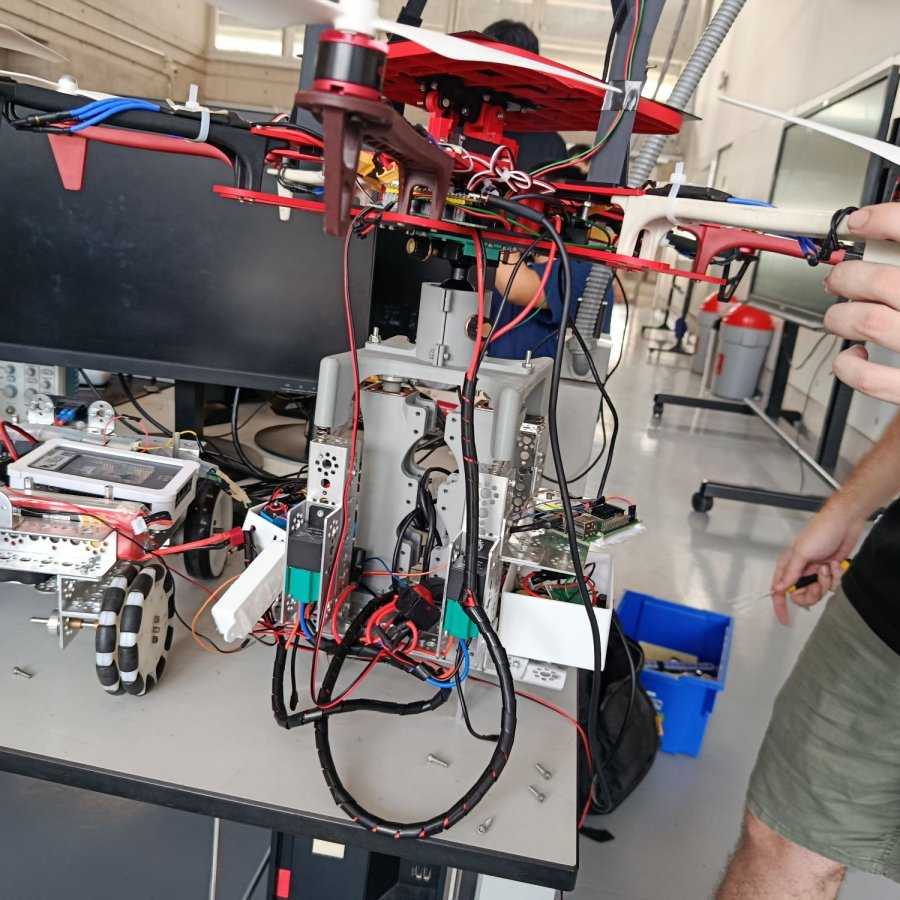
\includegraphics[width=\linewidth]{figures/paso4_dron_rotula.jpg}\caption{Step 4: drone mounted on the spherical joint.}\end{subfigure}\\[2mm]
  \begin{subfigure}[b]{0.24\textwidth}\centering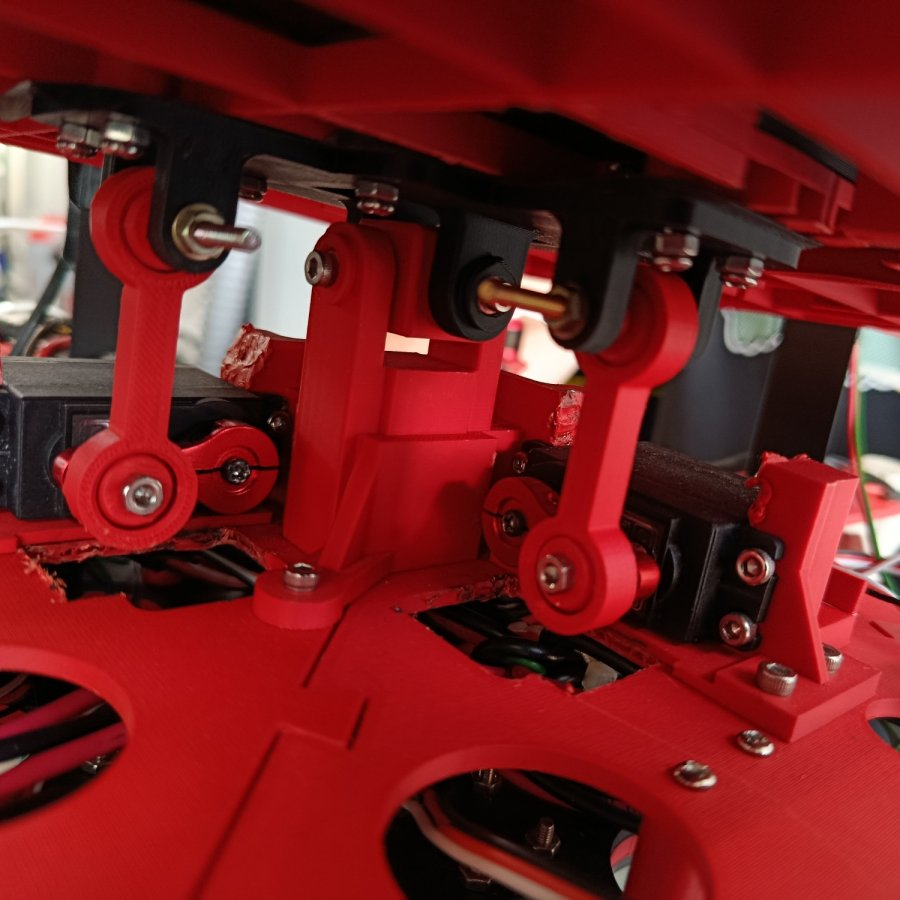
\includegraphics[width=\linewidth]{figures/paso5_mecanismo.jpg}\caption{Step 5: tray servos and linkages.}\end{subfigure}\hfill
  \begin{subfigure}[b]{0.24\textwidth}\centering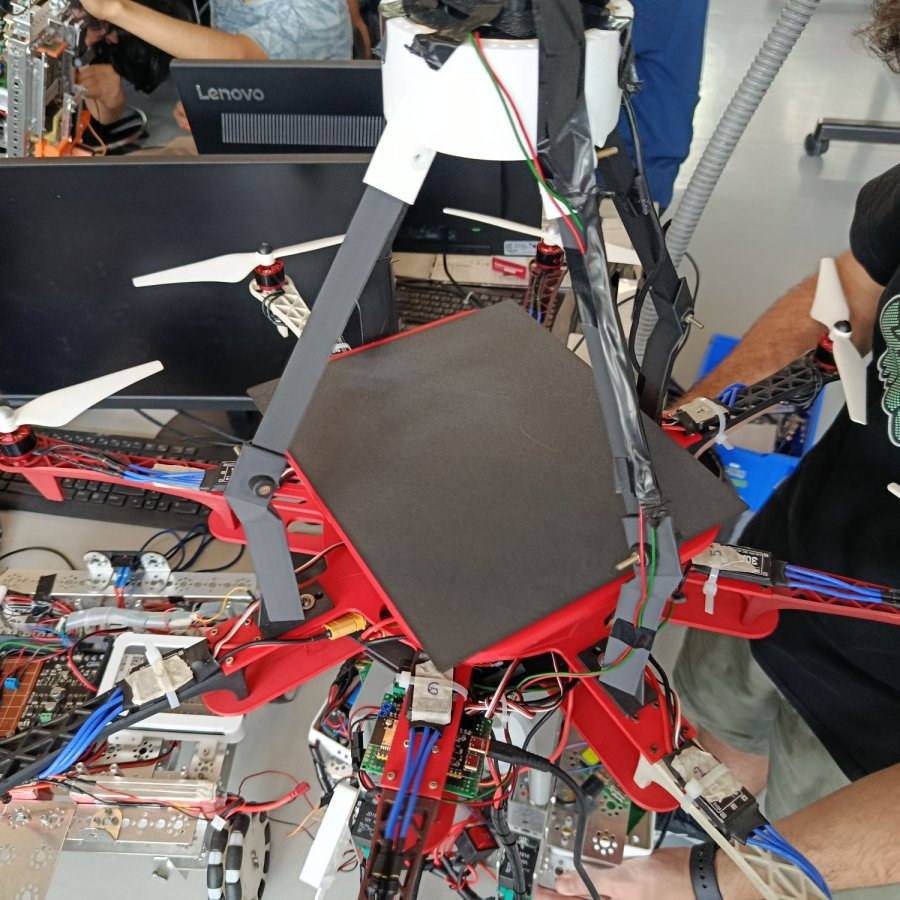
\includegraphics[width=\linewidth]{figures/paso5_bandeja_camara.jpg}\caption{Step 5: plate and camera towers.}\end{subfigure}\hfill
  \begin{subfigure}[b]{0.24\textwidth}\centering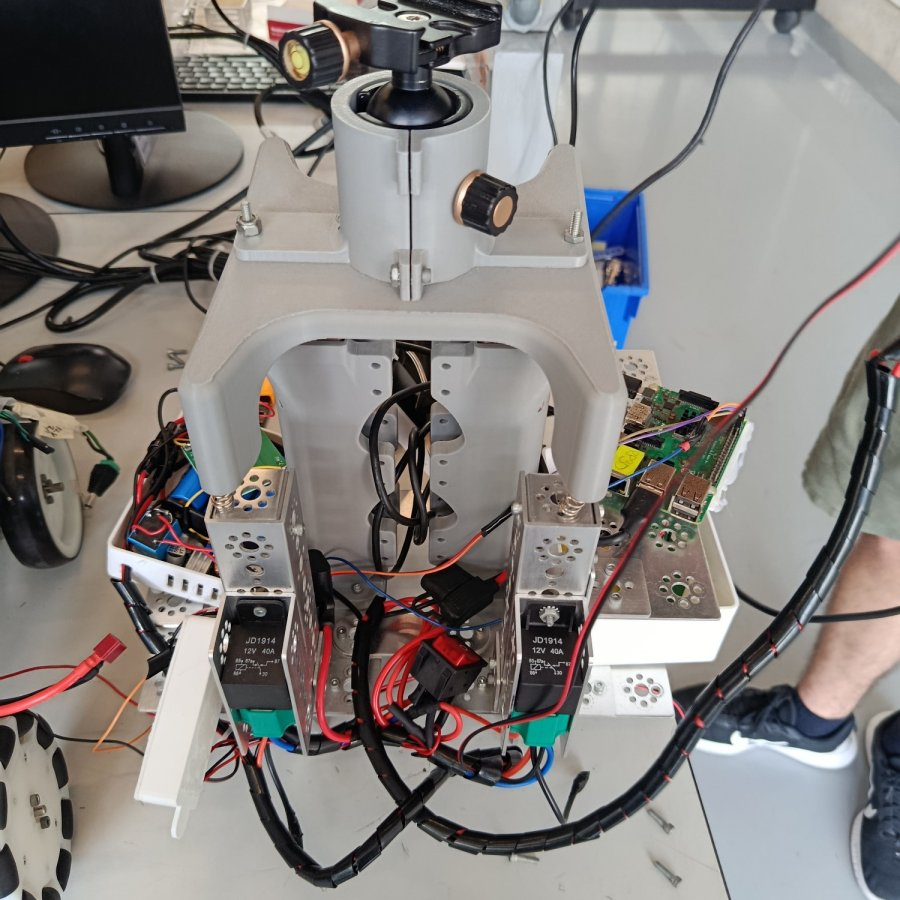
\includegraphics[width=\linewidth]{figures/paso6_supervisor.jpg}\caption{Step 6: emergency-stop relays and Raspberry Pi.}\end{subfigure}\hfill
  \begin{subfigure}[b]{0.24\textwidth}\centering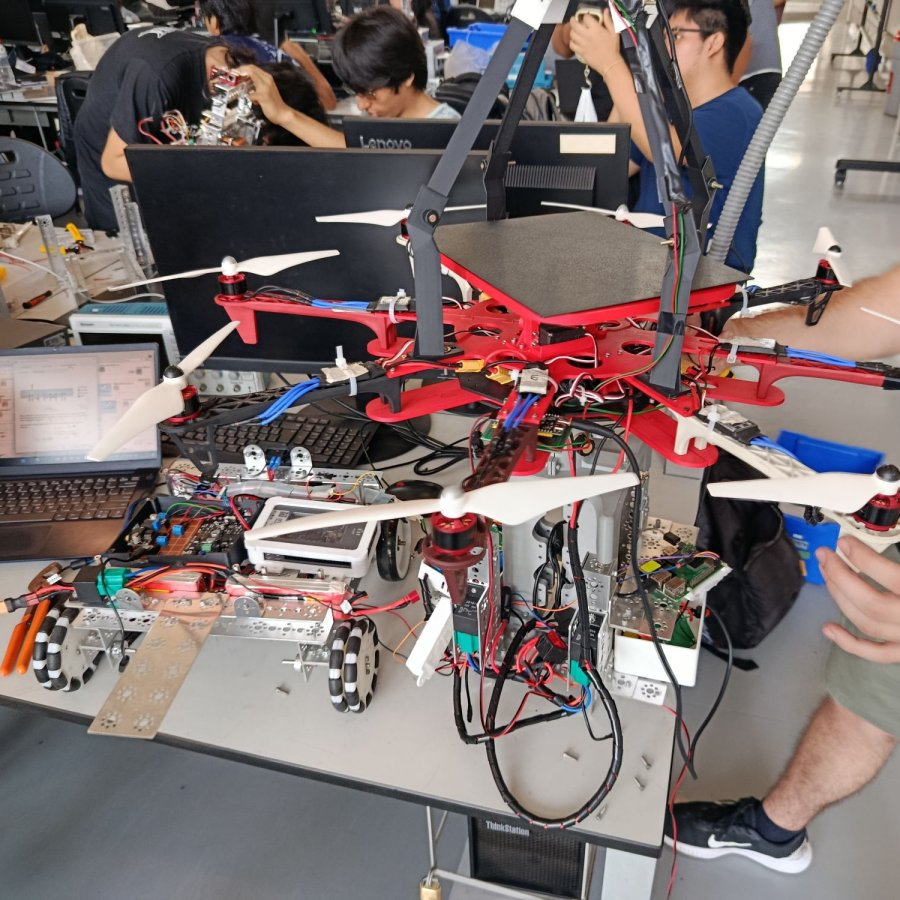
\includegraphics[width=\linewidth]{figures/paso7_integracion.jpg}\caption{Step 8: integration.}\end{subfigure}
  \caption{Build sequence of the final AeroTray prototype.}
  \label{fig:build}
\end{figure}

\begin{enumerate}[label=\textbf{Step \arabic*.}, leftmargin=*, align=left]
  \item \textbf{Mobile base (Fig.~\ref{fig:build}a).}
  \begin{enumerate}[label=(\alph*)]
    \item Assemble the TETRIX chassis with the two TorqueNADO motors on the rear axle and the omni wheels in front.
    \item Measure the track width (center-to-center distance between the drive wheels). It must match the value in the LabVIEW formula node, \SI{0.3794}{\metre}.
    \item Wire the left motor to myRIO MXP-A (PWM0 on pin 27, direction on DIO0, pin 11, encoder on ENC A/B) and the right motor to MXP-B on the same pins via the MDD10A.
    \item Protect the NiMH battery with the \SI{20}{\ampere} fuse and route it through the relay K3 contact.
    \item \emph{Check:} with the wheels off the ground, command forward motion and verify that both encoder counts increase. The right counter is inverted in software.
  \end{enumerate}

  \item \textbf{Mast, vertical guide, and spherical joint (Fig.~\ref{fig:build}b).}
  \begin{enumerate}[label=(\alph*)]
    \item Mount the vertical mast above the drive axle and attach the vertical guide.
    \item Insert the carriage with the spherical joint and verify approximately \SI{140}{\milli\metre} of free travel.
    \item Install soft end-stops at both ends of the guide.
    \item \emph{Check:} the carriage must drop freely under its own weight; guide friction biases the liftoff identification in Section~\ref{sec:ident}.
  \end{enumerate}

  \item \textbf{Octocopter frame and power (Fig.~\ref{fig:build}c).}
  \begin{enumerate}[label=(\alph*)]
    \item 3D-print the center plate and towers (file\\ \fn{x8_UAV_R350_imprimible_bandeja_v5.stp}) and mount the eight arms every \SI{45}{\degree}: M8 along $+x$, M7 along $+y$.
    \item Install M1--M4 as clockwise (CW) and M5--M8 as counterclockwise (CCW) (Table~\ref{tab:params}).
    \item Build the two independent power branches from the Rev.~I schematic (Section~\ref{sec:power}), each with a LiPo battery, XT60 connector, \SI{30}{\ampere} ATO fuse, relay contact 30--87 (K1, K2), 14\,AWG twisted pair, and a \SI{1000}{\micro\farad} capacitor at the drone. Branch A feeds ESCs 1, 3, 5, and 7; branch B feeds ESCs 2, 4, 6, and 8. Tie only the grounds together, and only at the drone.
    \item Cut the red (BEC) wire on all ESCs.
    \item Wire the ESC signals per Table~\ref{tab:pins} (firmware v11): NodeMCU-32S GPIO 25, 26, 27, 14, 21, 19, 5, and 17 for M1--M8; wire the MPU-6050 and VL53L0X to I$^2$C (SDA 23, SCL 22).
    \item Power the NodeMCU through the USB hub (logic domain). Do not add a regulator from the LiPo, as that would parallel two \SI{5}{\volt} supplies.
    \item Optional, recommended: solder VBAT voltage dividers to GPIO34/35 using R1 = R3 = \SI{10}{\kilo\ohm}, R2 = R4 = \SI{3.3}{\kilo\ohm} ($\div4.03$), and \SI{100}{\nano\farad} to GND so future firmware can measure battery voltage (Section~\ref{sec:bateria}).
  \end{enumerate}

  \item \textbf{Drone on the spherical joint (Fig.~\ref{fig:build}d).}
  \begin{enumerate}[label=(\alph*)]
    \item Bolt the frame to the spherical joint so the joint center coincides with the frame center.
    \item Balance the assembly so it sits level with the motors off. Shift the batteries until balanced and keep them as low as possible, because the center-of-mass height above the spherical joint sets the module's instability (Section~\ref{sec:limits_fund}). The prototype retains a \SI{9.5}{\milli\metre} residual eccentricity toward M8, identified in Section~\ref{sec:ident}.
  \end{enumerate}

  \item \textbf{Tray (Fig.~\ref{fig:build}e,f).}
  \begin{enumerate}[label=(\alph*)]
    \item 3D-print the plate, the linkages, and the four camera towers.
    \item Mount the two S3003 servos and connect their signal lines to GPIO47 ($x$) and GPIO21 ($y$) on the ESP32-S3.
    \item Power the servos from domain S5 (BT6, XL4015, relay K4 contact) with \SI{1000}{\micro\farad} at the input and a common ground with the ESP32-S3; do not connect the ESP32-S3 \SI{5}{\volt} pin to this rail.
    \item Mount the PS3 Eye on the towers, centered above the plate, and adjust the linkages so the plate sits level near \SI{1390}{\micro\second}.
  \end{enumerate}

  \item \textbf{Supervisor and emergency stop (Fig.~\ref{fig:build}g).}
  \begin{enumerate}[label=(\alph*)]
    \item Install Raspberry Pi OS (Debian 13) and create a virtual environment \texttt{\textasciitilde/venv} with \texttt{opencv-python}, \texttt{numpy}, \texttt{pyserial}, and \texttt{esptool}.
    \item Copy \texttt{pi\_control/} into the home directory.
    \item Enable the hardware UART: in \texttt{raspi-config}, set the serial login shell to \emph{No} and serial port hardware to \emph{Yes}, then reboot.
    \item Wire GPIO14 (TX, pin 8) to MXP-A pin 10 (RX), GPIO15 (RX, pin 10) to MXP-A pin 14 (TX), and GND (pin 6) to MXP-A pin 12.
    \item Power the Pi from its dedicated 3S 18650 pack (BT5) via an XL4015 set to \SI{5.2}{\volt}.
    \item Wire the control box: latching NC emergency-stop button SB1 in series with the K1--K4 coils powered from BT6 through a \SI{1}{\ampere} fuse, with a 1N4007 flyback diode across each coil. \emph{Check:} with SB1 pressed, no branch may have voltage downstream of its relay.
  \end{enumerate}

  \item \textbf{Firmware.}
  \begin{enumerate}[label=(\alph*)]
    \item Compile the drone firmware:\\ \texttt{arduino-cli compile --fqbn esp32:esp32:nodemcu-32s}.
    \item Flash it from the Pi using \fn{cargar_vuelo_guia_desde_pi.sh}, which runs \texttt{esptool write-flash 0x0}.
    \item Flash the ESP32-S3 with PlatformIO.
    \item Deploy the LabVIEW project to the myRIO (\fn{prueba_prueba.vi} as the main VI).
  \end{enumerate}

  \item \textbf{Integration checks (Fig.~\ref{fig:build}h).}
  \begin{enumerate}[label=(\alph*)]
    \item Launch \texttt{arrancar.sh} and open \url{http://<pi-ip>:8080/robot}. The log must display the drone firmware banner, \texttt{UART conectada en /dev/serial0} (UART connected), and the camera frame rate.
    \item With the battery disconnected, send \texttt{cal} and verify \texttt{CAL OK}.
    \item Place the ball on the plate and verify detection in all four corners.
  \end{enumerate}
\end{enumerate}
